\documentclass{report}

%\usepackage[latin1]{inputenc}
\usepackage[utf8x]{inputenc}
\usepackage[T1]{fontenc}
\usepackage[french]{babel}
\usepackage[cm]{fullpage}
\usepackage[pdftex]{graphicx}
\usepackage{setspace}
\usepackage{pgfgantt}
\usepackage{comment} 
\usepackage{amsmath}
\frenchbsetup{StandardLists=true}
\usepackage{enumitem}
\usepackage{tikz-uml}
\usepackage{url}
\usepackage{rotating}
<<<<<<< HEAD
\usepackage{hyperref}
=======
>>>>>>> 4661197567a56fb23484210dc9508a6e96f58acd

\sloppy
\hyphenpenalty 10000000
\definecolor{bargreen}{RGB}{133,193,132}
\definecolor{groupgreen}{RGB}{53,107,52}
\definecolor{darkgreen}{RGB}{35,68,35}
\definecolor{linkred}{RGB}{165,0,33}

\begin{document}

%page de garde
\begin{titlepage}

%logo de la fds, de l'UM et des infos

\includegraphics[scale=0.5]{logoFDS.png}
\hfill

\includegraphics[scale=0.2]{logoInfo.jpg}
\vspace{1cm}

\begin{center}
%au dessus du titre
\textsc{\Large{Rapport de projet T.E.R}} \\
\vspace{1cm}
\textsc{\Large{Projet Informatique HLIN405}} 
\vspace{1.5cm}

%titre
\doublespacing{\textsc{\huge{PunyDuck}}} \\
\vspace{2cm}

\includegraphics[scale=0.5]{logoPunyDuck.jpg}
\vfill
\end{center}

%noms/prenoms + Encadrante
\begin{minipage}[t]{8.5cm}
	\begin{flushleft}
	    \large{\textbf{Etudiants :}}
	    \begin{itemize}
	        \item \large{Valentin \bsc{FONTAINE}}
	        \item \large{Paul  \bsc{BUNEL}} 
	        \item \large{Esteban \bsc{BARON}}
	        \item \large{Valentin \bsc{PERON}}
	        \item \large{Julien \bsc{LEBARON}}
	    \end{itemize}
		\vspace{0.5cm}
		\large{\textbf{Encadrante :}}
		\large{Anne-Elisabeth \bsc{BAERT}} \\
	\end{flushleft}
\end{minipage}
\hfill
%année universitaire
\begin{minipage}[t]{8cm}
	\begin{flushright} 
		\large{\textbf{Année :}} 
		\large{2019-2020}
	\end{flushright}
\end{minipage}
\end{titlepage}

%Sommaire
\begin{titlepage}
\renewcommand{\contentsname}{Sommaire}
\setcounter{tocdepth}{1}
\large{\tableofcontents}
\thispagestyle{empty}
\end{titlepage}

%renommer les chapitres en parties
\renewcommand{\chaptername}{Partie}



%Introduction 1/2 pages
\chapter*{Introduction} %Partie présentation
\addcontentsline{toc}{chapter}{Introduction}
Dans le cadre du TER de notre deuxième année à la faculté des sciences de Montpellier nous avons proposé un projet s'intitulant PunyDuck. Le but de ce projet est la réalisation d'une plate-forme de distribution des projets des étudiants du département informatique.\\

Le groupe de développement est composé de cinq personnes, Valentin \textsc{FONTAINE}, Paul \bsc{BUNEL}, Valentin \bsc{PERON}, Julien \bsc{LEBARON} et Esteban \bsc{BARON}. Nous sommes encadré par Mme Anne-Elisabeth \bsc{BAERT}.

\section*{Motivation}

Le TER est un module qui apporte beaucoup aux étudiants en gestion de projet ainsi qu'en programmation. Seulement une fois terminés les projets ne sont pas valorisés et tombent dans l'oubli. Notre solution est de proposer une application permettant à chaque étudiants de déposer leurs projets pour les rendre visibles et téléchargeables par tous.

\section*{Approches}
Notre objectif final étant de produire une application fonctionnelle pouvant être utilisée par tous, nous avions besoin : d'une interface graphique décente, totalement opérationnelle et facilement modulable, ainsi que d'un système de communication efficace entre l'application et une base de donnée. Nous avons donc décidés de diviser le projet en trois partie : tout d'abord la conception d'un framework permettant la réalisation d'interfaces graphiques, puis la réalisation de l'interface graphique elle-même à partir de ce framework, et enfin la partie réseau permettant à l'application de communiquer avec un serveur distant. Ces trois parties communiquent ensembles part le biais d'une architecture logiciel MVC (Modèle-Vue-Contrôleur).\\
Notre appplication est téléchargeable par tous depuis le site web \url{ https://fvostudio.com/punyduck/}.

\section*{Cahier des charges}
Le but de Punyduck est de proposer aux étudiants en informatique une plateforme de distribution de leurs différents projets. Cette plateforme devait être une application téléchargeable sur un site internet, et connectée à un serveur pour permettre l'échange de projets entre différents clients. \\
Pour l'organisation du projet, nous l'avons tout d'abord divisé en plusieurs étapes : 
\begin{itemize}[label=$-$]
    \item Mise en place d’un serveur qui servira d’intermédiaire entre les utilisateurs et la base de données.
    \item Création d’un framework pour faciliter la réalisation de l’application.
    \item Conception de l’application graphique à l’aide du framework.
    \item Connexion entre l’application graphique et le serveur.
    \item Création d’une base de données pour stocker les comptes des utilisateurs et les
projets.
    \item Mise en service d’un site internet permettant le téléchargement de l’application.
\end{itemize}
\newpage
Ensuite, une fois les différentes parties du projet dégagées, pour bien définir chacune d'entre elles nous avons décidé du cahier des charges suivant :
\begin{description}
%I 
    \item[Le serveur :] Le serveur devra fonctionner de manière asynchrone (nous définiront ce principe dans la prochaine partie). Il pourra héberger de manière sécurisée les données des utilisateurs (nom, mots de passes, ...) et devra être capable de gérer la plupart des erreurs de réseau, comme les coupures de connexion lors d'un téléchargement.
%II
    \item[Le framework :] Le framework définira un ensemble de classes et fonctions qui serviront de base à la structure d'une nouvelle application. Son utilisation doit être facile avec assez de fonctionnalités déjà disponibles pour pouvoir réduire les appels de fonctions bas niveau. De plus, il devra également permettre la plasticité des interfaces.
%III
    \item[L’application :] Notre application présentera une interface graphique permettant de naviguer facilement entre différents onglets, de communiquer avec le serveur, et de personnaliser un minimum l'apparence : mode clair / sombre, position de certains éléments de la fenêtre, couleur de l’arrière plan.
%IV
    \item[La base de données :] Elle stockera les données relatives aux comptes des utilisateurs ainsi que les projets. Les données confidentielles (mots de passe) seront cryptées.
%V
    \item[Le site :] Il sera constitué d'une unique page permettant de télécharger l'application. Il possèdera un design « responsive~ » et dynamique.
\end{description}

%Quelques définitions ici comme dans l'exemple de rapport ?

%Partie 2 Partie technologies utilisées 1/2 pages
\chapter{Technologies utilisées}
\section{Langages}
 % idées à reformuler
Pour la programmation de notre application, nous avons choisis assez naturellement d'utiliser le langage C/C++. En effet, c'est le langage que nous avons le plus étudié à l'université, avec lequel 3 des 5 membres du groupe avaient codé leur projet de Licence 1 CMI, et qui nous offrait un support puissant et efficace pour notre interface graphique. \\
De plus le C++ nous a permis de coder en orienté objet, ce qui était une nécessitée pour la création de notre application. En effet, notre programme utilise énormément ce type de programmation : nous développeront ce point plus tard dans la partie 3 sur le développement logiciel. \\

Pour l'interface graphique, nous avons utilisé la bibliothèque OpenGL : une interface regroupant environ 250 fonctions différentes qui peuvent être utilisées pour afficher des scènes tridimensionnelles complexes à partir de simples primitives géométriques. Du fait de son ouverture, de sa souplesse d'utilisation et de sa disponibilité sur toutes les plates-formes, OpenGL est une des bibliothèque graphiques les plus utilisée par la majorité des applications scientifiques, industrielles ou artistiques 3D. \\
L'utilisation de cette bibliothèque (associée à GLFW pour la gestion des fenêtres) était donc un choix assez basique puisqu'elle est très répandue, mais nous avons dû apprendre à l'utiliser : celle-ci est beaucoup plus complexe que les librairies que nous avions utilisées auparavant, comme SFML ou PyGame, de par son bas niveau. \\

Pour gérer la partie réseau de notre application, nous n'avions pas besoin d'utiliser un langage puissant comme le C/C++, nous pouvions donc nous rabattre sur un langage moins performant mais plus facile d'accès.
De ce fait, nous nous sommes dirigés vers le langage python, qui est un langage très simple d'utilisation, pratique pour débuter dans le domaine complexe de la programmation que représente la programmation en réseau. De surcroît il est plutôt efficace pour gérer les entrées sorties, notamment pour la lecture et l'écriture dans des fichiers, qui est une notion centrale dans notre projet.\\

Cependant, le langage Python de base ne permet pas de faire de la programmation en réseau, nous avons donc du choisir une des nombreuses bibliothèques disponibles permettant de faire de la programmation réseau en Python. Après réflexion, nous avons opté pour le module « asyncio » pour deux raisons : premièrement, ce module offrait une interface de programmation en réseau de haut niveau donc plus simple d'utilisation, ce qui nous arrangeait particulièrement étant donné que nous sommes parfaitement novices dans ce domaine ; Deuxièmement, le gros point fort de ce module est le fait qu'il implémente une nouvelle manière de programmer~: la programmation asynchrone. La programmation asynchrone pour les entrées/sorties est une forme de programmation parallèle permettant d'exécuter d'autres parties d'un programme lorsque celui-ci est en attente d'une transmission de donnée, afin de grandement diminuer le temps d'exécution du programme. \\

\section{Outils} %outils utilisés pourquoi ce choix avantages ? postgresql
Pour réaliser notre projet nous avons utilisé des outils différents et spécifiques à chaque tache. \\

Nous avons utilisé le système de gestion PostgreSQL\footnote{PSQL : \url{https://www.postgresql.org/}} pour gérer la base de donnée de notre serveur, ce système nous permettant d'utiliser des requête SQL en Python et ainsi de mettre en application les connaissances acquises cette année avec le module HLIN304. \\

Pour la partie modélisation de l'application nous avons opté pour le Langage de Modélisation Unifié (UML) vu en cours, dans le module HLIN406. \\

Toutes les communications du groupe ce sont faites sur le logiciel Discord\footnote{Discord : \url{https://discordapp.com/}}, un logiciel facilitant grandement les communications en groupes avec par exemple le partage d'écran, les groupes vocaux et textuels, le fait de pouvoir partager des morceaux de code directement dans le canal de discussion textuel etc.. \\

Pour ce qui est du partage et des sauvegardes du code, nous avons utilisé Git (un logiciel de gestion de versions décentralisé) via un serveur GitHub\footnote{GitHub \url{https://github.com/}, notre projet : \url{https://github.com/valfvo/punyduck}} qui nous a permis de garder nos anciennes versions, de ne rien perdre en cours de route, et de pouvoir partager l'avancée du projet avec les autres étudiants du groupes et notre encadrante. \\

Pour ce qui est de l'éditeur de code utilisé, nous nous sommes tous penché sur Visual Studio Code\footnote{VSCode : \url{https://code.visualstudio.com/}} pour sa fiabilité et sa mise en page agréable. De plus, nous avons pu grâce à ce logiciel coder à plusieurs en même temps avec sa fonctionnalité de partage en temps réel. \\

Enfin, nous avons utilisé le langage \LaTeX{} via la plateforme Overleaf\footnote{Overleaf : \url{https://www.overleaf.com/}} pour rédiger ce rapport.


%Partie 3 Développement logiciel 5/10 pages
\chapter{Développement logiciel, Conception, Modélisation, Implémentation}
\section{Présentation du développement}
Le développement du projet est séparé en trois parties : 
\begin{itemize}[label=$-$, leftmargin=1.5cm]
    \item le framework de l'interface graphique ;
    \item l'interface graphique utilisant le framework ;
    \item la communication réseau entre le client et le serveur.
\end{itemize}

Le développement de l'application s'est déroulé en plusieurs étapes qui vont être développées points par points.

\subsection{Apprentissage de l'utilsiation d'OpenGL}
La première étape fut d'apprendre l'OpenGL, qui fut difficile à comprendre et à utiliser de par son bas niveau comparé aux librairies qu'on a l'habitude de voir en L1 et L2. \\
La première partie de l'apprentissage d'OpenGL a été de pour dessiner un triangle d'une certaine couleur. Puis grâce à ce triangle de pouvoir dessiner un rectangle. Ainsi de suite nous avons pu dessiner toutes sortes de formes tel que les ronds et les cercles par exemple.
La deuxième partie a été de pouvoir coller des textures sur ces surfaces précédemment créées. Cette partie n'a pas posé réellement de problème.
Pour la troisième partie, nous devions pouvoir mettre une surface dans une autre surface, comme dans la figure \ref{exsurface}.
\begin{figure}
    \begin{center}
        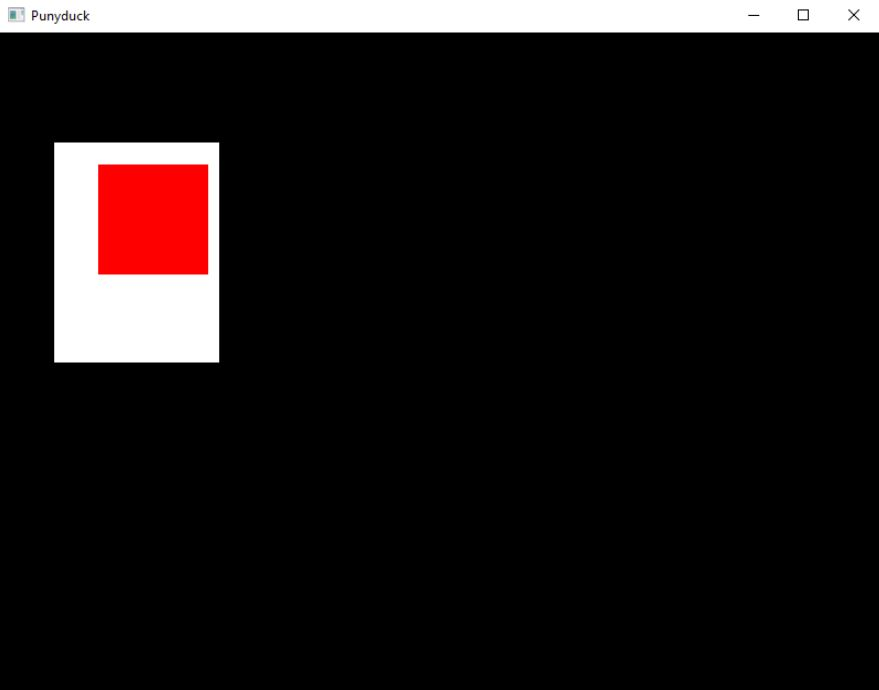
\includegraphics[scale=0.3]{exempleSurface.jpg}
        \caption{Capture d'écran de notre premier essai d'une superposition de surfaces}
        \label{exsurface}
    \end{center}
\end{figure}
Ceci était primordial pour la réalisation de l'application graphique car cette simple tache à permis la superposition des éléments graphiques de l'application. \\
%plus argumenter sur le texte
La dernière partie était de créer le texte, c'est-à-dire de pouvoir afficher du texte à l'écran. \\

La seconde étape du développement de l'application a été de modéliser en UML les différentes parties de l'application et ses mécanismes. \\
%mieux argumenter ici
Pour commencer il fallait trouver un système permettant de lier des éléments entre eux afin de pouvoir les superposer, créer de nouveaux éléments à partir d'anciens, de supprimer un élément et ses sous éléments qui le compose etc..
C'est pour cela que nous avons créé les "Quarks", un système où un élément a un  père et n fils (où n appartient à l'intervalle \(\left]0, +\infty\right[\)) et a accès à ses frères. Grâce à ce mécanisme, tous les problèmes cité précédemment ont été résolus. Ce système a donc été la base de toute l'application. \\
Ensuite nous avons créé les différentes classes qui allaient nous servir pour l'implémentation. Comme par exemple : 
%FAIRE LES EXPLICATIONS SUR LES CLASSES COMPLEXES ET SI BESOIN RAJOUTER D'AUTRES CLASSES 
\begin{itemize}
    \item "LQTexture" qui génère les textures
    \item "LQSurface" pour les surfaces
    \item "LQViewable" 
    \item "LQColor" pour la couleur
    \item "LQNumber" 
    \item "LQText" pour le texte
    \item "LQButton" pour les boutons 
\end{itemize}

%plus argumenter ici
La troisième étape fut la phase d'implémentation. D'une part nous nous sommes occupés des classes en rapport avec d'OpenGL tels que "LQShader", "LQTexture" et "LQSurface".
Par la suite nous avons coder les différentes classes en suivant l'UML précédemment réalisé.

%ici jvous laisse faire jsp du tt quoi mettre
Pour le côté serveur et base de donnée la première étape fut de ...

\section{Modélisation} %UML gros problème. dès que l'on rajoute des lignes, tout crash avec trois milles erreurs.
%Incompréhensible, peux-être parce que sa déborde je n'ai pas trouver malgré plusieurs essaies.
%Je les remplis et après il faudra voir comment les placer pour pas que ça plante
%Le problème provient sûrement quand un umlclass déborde sur un autre. /!\

\begin{center}
\begin{tikzpicture}
\umlclass[x=-1,y=-10, fill=gray!5]{LQSurface}{
    -- m\_VBO : GLuint\\
    -- m\_VAO : GLuint\\ 
    -- m\_FBO : GLuint\\
    -- m\_shader : LQShader\\ 
    -- m\_x : LQNumber\\
    -- m\_y : LQNumber\\ 
    -- m\_width : LQNumber\\ 
    -- m\_height : LQNumber\\ 
    %les trois du bas font tout planter peux importe où tu les mets
    %-- m\_clearColor : LQColor\\
    %\umlstatic{-- s\_vertices[54] : GLfloat}\\
    %\umlstatic{-- s\_default\_shader : LQShader}
    }{
<<<<<<< HEAD
    + blit(LQTexture texture, GLfloat x, GLfloat y, GLuint VAO) : void\\
    + fill(GLfloat r, GLfloat g, GLfloat b, GLfloat a=1.0f) : void\\
    + blit(const LQSurface surface) : void\\
    + fill(LQColor color) : void\\
=======
    + blit(LQTexture const& texture, GLfloat x, GLfloat y, GLuint VAO) : void\\
    + fill(GLfloat r, GLfloat g, GLfloat b, GLfloat a=1.0f) : void\\
    + blit(const LQSurface& surface) : void\\
    + fill(LQColor const& color) : void\\
>>>>>>> 4661197567a56fb23484210dc9508a6e96f58acd
    + move(GLfloat x, GLfloat y) : void\\
    + move(glm::vec2 distance) : void\\
    + moveX(GLfloat x) : void\\
    + moveY(GLfloat y) : void\\
    + moveTo(GLfloat x, GLfloat y) : void\\
<<<<<<< HEAD
    + moveTo(glm\::vec2 position) : void\\
=======
    + moveTo(glm::vec2 position) : void\\
>>>>>>> 4661197567a56fb23484210dc9508a6e96f58acd
    + moveToX(GLfloat x) : void\\
    + moveToY(GLfloat y) : void\\
    }

\umlclass[x=-5, fill=gray!5]{LQuark}{
    -- m\_parent : LQuark \\
    -- m\_prevSibling : LQuark \\
    -- m\_nextSibling : LQuark \\
    -- m\_firstChild : LQuark \\
    -- m\_lastChild : LQuark \\
    %-- m\_childrenCount : LQuark \\
    }{
    + <<create>>LQuark() \\
    + parent() : LQuark \\
    + firstChild() : LQuark \\
    + lastChild() : LQuark \\
    %+ nthChild(LQindex nth) : LQuark \\
    + prevSibling() : LQuark \\
    + nextSibling() : LQuark \\
    %+ nthSibling(LQindex nth) : LQuark \\
    %+ childrenCount() : LQsize \\
    %+ setNextSibling(LQuark nextSibling): void \\
    + appendChild(LQuark child) : LQuark \\
    %+ insertChild(LQindex index, LQuark child) : LQuark \\
    %+ insertChildBefore(LQuark newChild, LQuark child) : LQuark \\
    %+ insertChildAfter(LQuark newChild, LQuark child) : LQuark \\
    %+ detach() : LQuark \\
    + removeChild(LQuark child) : LQuark \\
    %+ removeFirstChild() : LQuark \\
    %+ removeLastChild() : LQuark \\
    %+ removeChildren(LQuark newParent) : LQuark \\
    %+ swapWith(LQuark quark) : LQuark \\
    %+ swapChildren(LQuark first, LQuark second) : LQuark \\
    %+ swapChildren(LQindex first, LQindex second) : LQuark}
}
\umlclass[x=4.5, fill=gray!5]{LQTexture}{
    -- m\_id : GLuint \\
    -- m\_texWidth : GLuint \\
    -- m\_texHeight : GLuint \\
    -- m\_format : GLuint \\
    -- m\_wrapS : GLuint \\
    -- m\_wrapT : GLuint \\
    -- m\_minFilter : GLuint \\
    -- m\_magFilter : GLuint}{
    + <<create>>LQTexture(string path, int width, int height) \\
    + <<create>>LQTexture(LQTexture other) \\
    + <<create>>LQTexture()\\
    -- genTexture(): GLuint \\
    -- resize(GLuint texWidth, GLuint texHeight):LQTexture\\
    + getId(): GLint \\
    + getWidth(): GLint \\
    + getHeight(): GLint \\
    \umlstatic{+ deleteTexture(LQTexture texture): void}
}

%lien entre bloc
\umlinherit[geometry=-|]{LQuark}{LQSurface}
\umlinherit[geometry=-|]{LQTexture}{LQSurface}
\end{tikzpicture}
\end{center}

\begin{center}
\begin{tikzpicture}
\umlclass[fill=gray!5]{LQNumber}{
    -- m\_quark : LQuark\\
    %-- (*m\_invoke)(LQuark*) : void \\ Trouver comment représenter une fonction en attribut UML
    -- m\_value : float \\
    -- m\_kind : Kind\\
    -- m\_expr : LQMathExpr \\
    -- m\_refs : forward\_list<LQNumber*> \\
    \umlstatic{-- s\_old : float}
}{
    + Kind : enum class ({value,length,coords})\\
    + <<create>>LQNumber() \\
    + <<create>>LQNumber(float value) \\
    + <<create>><<create>>LQNumber(LQMathExpr expr) \\
    + <<create>>LQNumber(Kind kind) \\
    + <<create>>LQNumber(LQNumber other) \\
    + linkQuark(TQuark quark) : void \\
    + recalc() : void \\
    + removeRef(LQNumber ref) : void \\
    + i() : float \\
    + f() : float \\
    + float() : operator \\
    \umlstatic{+ old() : float}
    }
\umlclass[y=-8, fill=gray!5]{LQMathVar}{
    -- m\_number : LQNumber \\
    -- m\_coeff : float \\
    -- m\_next : LQMathVar
}{
    + <<create>>LQMathVar(LQNumber number, float coeff=1.0f)\\
    + setNext(LQMathVar next) : void \\
    + eval() : float \\
    + parentCoords(LQNumber number) : bool \\
    + compatible(LQNumber number) : bool
}
\umlclass[x=10, y=-10, fill=gray!5]{LQMathExpr}{
    -- addCompatible(LQMathVar first, float coeff=1.0f) : void\\
    -- m\_first : LQMathVar \\
    -- m\_last : LQMathVar \\
    -- m\_constant : float \\
}{
%    + <<create>>LQMathExpr()\\
    + <<create>>LQMathExpr(LQNumber number)\\
    + <<create>>LQMathExpr(LQMathExpr other)\\
    + eval() : float \\
    + reset() : void \\
    \umlvirt{+ operator=(float constant) : LQMathExpr <<operator>>}\\
    \umlvirt{+ operator=(LQMathExpr expr) : LQMathExpr <<operator>>}\\
    \umlvirt{+ operator+=(float constant) : LQMathExpr <<operator>>}\\
    \umlvirt{+ operator-=(float constant) : LQMathExpr <<operator>>}\\
    \umlvirt{+ operator*=(float coeff) : LQMathExpr <<operator>>}\\
    \umlvirt{+ operator/=(float coeff) : LQMathExpr <<operator>>}\\
    \umlvirt{+ operator+(float constant) : LQMathExpr <<operator>>}\\
    \umlvirt{+ operator+(LQMathExpr other) : LQMathExpr <<operator>>}\\
    \umlvirt{+ operator-(float constant) : LQMathExpr <<operator>>}\\
    \umlvirt{+ operator-(LQMathExpr other) : LQMathExpr <<operator>>}\\
    \umlvirt{+ operator*(float coeff) : LQMathExpr <<operator>>}\\
    \umlvirt{+ operator/(float coeff) : LQMathExpr <<operator>>}
    }
%lien
\umlinherit[geometry=-|]{LQMathVar}{LQMathExpr}
\umlinherit[geometry=|-]{LQMathExpr}{LQNumber}
\end{tikzpicture}
\end{center}

\begin{center}
\begin{tikzpicture}
\umlclass[fill=gray!5]{LQViewable}{
    -- m\_flex : bool\\ 
    -- m\_hidden : bool
}{
    %+ <<create>>LQViewable();\\
    + <<create>>LQViewable(LQNumber x, LQNumber y,
               LQNumber width, LQNumber height,\\
               GLint color=0x000000, const std::string iconPath="")\\
    %+ <<create>>LQViewable(LQNumber x, LQNumber y, bool flex=true)\\
    %+ hidden() : bool\\ 
    + hide() : void\\
    + unhide() : void\\
    %+ flexible() : bool\\ 
    + displayFlex() : void\\
    %+ displayBlock() : void\\
    + appendChild(LQViewable child) :  LQViewable\\ 
<<<<<<< HEAD
    + drawChildren() : void \\
    + resizeWidthCallback() : void\\
    \umlvirt{+ resizeHeightCallback() : void}
}
\umlclass[x=-3, y=-5, fill=gray!5]{LQSurface}{...}{...}
\umlclass[x=3, y=-5, fill=gray!5]{LQNumber}{...}{...}
=======
    + ^drawChildren() : void \\
    + resizeWidthCallback() : void\\
    \umlvirt{+ resizeHeightCallback() : void}
}
\umlclass[x=-3, y=-5, fill=grey!5]{LQSurface}{...\\}{...\\}
\umlclass[x=3, y=-5, fill=grey!5]{LQNumber}{...\\}{...\\}
>>>>>>> 4661197567a56fb23484210dc9508a6e96f58acd
\umlinherit[geometry=-|]{LQNumber}{LQViewable}
\umlinherit[geometry=-|]{LQSurface}{LQViewable}
\end{tikzpicture}
\end{center}

\section{Fonctionnalités de l'interface}
%Je parle de ce qui devait être fait (j'ai pas mis les notification, ni personnalisation) si quelque chose ne peux être fait ou n'est pas fait d'ici la fin, enlever directement la partie en question.
L'interface graphique est composé de plusieurs fenêtres, chacune spécifique. D'autant plus que l'ensemble peux être personnalisable (placement de certains bloc présent sur l'interface). Pour la partie commune à chaque fenêtre de l'interface
on a la barre des onglets contenant, dans cet ordre :
\vspace{0.5cm}
\begin{itemize}
    \item "L'accueil", comprenant les lancements rapide d'application dernièrement utilisées ainsi que les nouveautés lié à l'application ou de certains projets.
    \item Les "Projets", où l'ensemble des projets mis en ligne seront affichés. 
    %\item La "Collection", contenant les projets suivie et télécharger seront directement affichés.
    \item Le "Profil" est l'endroit où l'on peut modifier ses données personnelles, sa page de profil et les paramètres de l'application.
    %\item Les "Contact", seront les différentes personnes suivie ou qui nous suive avec la possibilités d'échanger par message dans l'application.
    %\item La "Communauté" recensera l'ensemble des forums d'aides.
    \item Le "Dépôt" vas servir à faire une demande de dépôt de projet, afin qu'il soit vérifier avant mise en ligne (pour éviter les dépôt de virus ou autre).
    \item Icônes basique tel que épinglé, réduire et fermer. Mais contient aussi le mode nuit (fond clair qui devient foncé).
\end{itemize}
\vspace{0.5cm}
La fonctionnalité principale étant d'aller sur la page projet, voir un qui nous intéresse ou faire une demande de dépôt pour notre projet. Maintenant cas par cas voyons les différentes interactions.\\
Pour l'accueil il est possible de cliquer sur les articles mis en avant enfin de pouvoir les lires en détails, mais aussi les lancements rapides des derniers projet lancer en cliquant sur l'icône en question. Pour les projets, les fonctionnalitées qui changes sont les touches de tri et d'affichage ainsi que la barre rechercher. Pour la collection, c'est pareil sauf que l'on peux acceder à un menu d'action a coté de chaque projet (ressemblant à 3 petit points):
\begin{itemize}
    \item Désinstaller
    \item Emplacement
    \item Page projet
    \item Désabonner / Ne plus suivre
\end{itemize}
Ainsi que les boutons d'action, lancer qui vas démarrer l'application, et installer qui vas télécharger et installer l'application.\\
En ce qui concerne la page de présentation du projet, on peux interagir avec la notations (données une notes ou envoyé un commentaire) mais également un lien qui va envoyé vers un forum existant en lien avec le projet. On a notamment accès au bouton suivre pour l'avoir dans notre collection et le bouton j'aime pour aimé un projet.\\
Les interactions avec l'interface concernant le profil sont, la modification de fond et de l'image de profil ainsi que des autres paramètres (nom, prénom, mot de passe,...), l'accès au paramètre du client (langue,emplacement,...) et le bouton de déconnexion.

\section{Format des données et procédure d'utilisation} % dnnées utilisées ou encore convention, décrire certaines procédures de lecture et de validation
\section{Statistique} %nombres de classes/scripts/ lignes de code/ nombre de module

%Partie 4 
\chapter{Algorithmes et Structures de Données}
\section{Présentation des principales structures de données}
\section{Présentation des principaux algorithmes}%présentation et description de deux ou un algo très important et intéressant 
\section{Complexité théorique}

%.Partie 5 1/2 pages
\chapter{Gestion du Projet}
\section{Organisation et planification}
\newpage
\begin{rotate}{270}
\begin{comment}
%police du gantt au choix selon préférence
\definecolor{bargreen}{RGB}{133,193,132}
\definecolor{groupgreen}{RGB}{53,107,52}
\definecolor{darkgreen}{RGB}{35,68,35}
\definecolor{linkred}{RGB}{165,0,33}

\renewcommand\sfdefault{phv}
\renewcommand\mddefault{mc}
\renewcommand\bfdefault{bc}

\setganttlinklabel{s-s}{START-TO-START}
\setganttlinklabel{f-s}{FINISH-TO-START}
\setganttlinklabel{f-f}{FINISH-TO-FINISH}
\begin{ganttchart}[
    canvas/.append style={fill=none, draw=black!25, line width=3pt},
    hgrid style/.style={draw=black!5, line width=.75pt},
    vgrid={*1{draw=black!5, line width=.75pt}},
    x unit=0.85cm,
    today label font=\small\bfseries,
    title/.style={draw=none, fill=none},
    title label font=\bfseries\footnotesize,
    title label node/.append style={below=7pt},
    include title in canvas=false,
    %Zone des sous parties d'un groupe
    bar label font=\mdseries\small\color{black!90},
    bar label node/.append style={left=1cm},
    bar/.append style={draw=none, fill=darkgreen!60},
    bar incomplete/.append style={fill=bargreen},
    bar progress label font=\mdseries\footnotesize\color{black!70},
    %tête de groupe (Réseau, framwork)
    group incomplete/.append style={fill=groupgreen!85},
    group/.append style={draw=none, fill=darkgreen},
    group left shift=0,
    group right shift=0,
    group height=0.3,
    group peaks tip position=0,
    group label node/.append style={left=1.5cm},
    group progress label font=\bfseries\small,
    %zone rouge / avancement
    link/.style={-latex, line width=1.5pt, linkred},
    link label font=\scriptsize\bfseries,
    link label node/.append style={below left=-1pt and 0pt}
  ]{1}{15}
  \gantttitle[
    title label node/.append style={below left=7pt and -3pt}
  ]{SEMAINES:\quad1}{1}
  \gantttitlelist{2,...,15}{1} \\
  \ganttgroup{Préliminaire Projet}{1}{1} \\[grid]
  \ganttgroup[name = R]{Partie Réseaux}{2}{10} \\
  \ganttbar[progress=75,name=PR1A]{\textbf{PR 1.1} Activité A}{2}{8} \\
  \ganttbar[progress=67,name=PR1B]{\textbf{PR 1.2} Activité B}{2}{10} \\
  \ganttbar[progress=0 ,name=PR1C]{\textbf{PR 1.4} Activité C}{4}{10} \\[grid]
  \ganttgroup{Partie framework}{2}{10} \\
  \ganttbar[progress=0]{\textbf{PFRA 2.1} Activité D}{2}{5} \\
  \ganttbar[progress=0]{\textbf{PFRA 2.2} Activité E}{3}{5} \\
  \ganttbar[progress=0]{\textbf{PFRA 2.3} Activité F}{4}{5}\\[grid]
  \ganttgroup[name= F]{Partie frontwork}{11}{14} \\
  \ganttbar[progress=0]{\textbf{PFRO 2.1} Activité G}{5}{6} \\
  \ganttbar[progress=0]{\textbf{PFRO 2.2} Activité H}{6}{8} \\
  \ganttbar[progress=0]{\textbf{PFRO 2.3} Activité I}{9}{10}\\[grid]
  \ganttgroup{Partie Rapport}{2}{15}\\[grid]
  \ganttgroup{Partie Site web}{9}{13}
  
  %link entre activitées
  \ganttlink[link type=s-s]{PR1A}{PR1B}
  \ganttlink[link type=f-s]{R}{F}
  \ganttlink[link type=f-f,link label node/.append style=left]{PR1C}{PR1B}
\end{ganttchart}
\end{comment}
%\begin{comment}
\setganttlinklabel{s-s}{START-TO-START}
\setganttlinklabel{f-s}{FINISH-TO-START}
\setganttlinklabel{f-f}{FINISH-TO-FINISH}
    \begin{ganttchart}[
        hgrid,
        vgrid={*{6}{draw=none},{dotted}},
        vrule/.style={very thick, red},
        x unit=0.160cm,
        time slot format=isodate,
        time slot unit=day,
        calendar week text = {W\currentweek{}},
        bar height = 0.6,
        bar top shift = 0.2,
        bar label node/.append style={align=left,text width={width("Task1 ")}},
        bar incomplete/.append style={fill=cyan},
        progress label text = \relax
        link/.style={-latex, line width=1.5pt, linkred},
        ]{2020-02-01}{2020-05-30}
        \gantttitlecalendar{year, month=name, week} \\
        \ganttbar[bar/.append style={fill=bargreen}]{Task1}{2020-02-01}{2020-02-05}\\
        \ganttbar[bar/.append style={fill=bargreen}]{Task1}{2020-02-01}{2020-02-05}\\
        \ganttbar[bar/.append style={fill=bargreen}]{Task1}{2020-02-01}{2020-02-05}\\
        \ganttbar[bar/.append style={fill=bargreen}]{Task1}{2020-02-01}{2020-02-05}\\
        \ganttbar[bar/.append style={fill=bargreen}]{Task1}{2020-02-01}{2020-02-05}\\
        \ganttbar[bar/.append style={fill=bargreen}]{Task1}{2020-02-01}{2020-02-05}\\
        \ganttbar[bar/.append style={fill=bargreen}]{Task1}{2020-02-01}{2020-02-05}\\
        \ganttbar[bar/.append style={fill=bargreen}]{Task1}{2020-02-01}{2020-02-05}\\
        \ganttbar[bar/.append style={fill=bargreen}]{Task1}{2020-02-01}{2020-02-05}\\
        \ganttbar[bar/.append style={fill=bargreen}]{Task1}{2020-02-01}{2020-02-05}\\
        \ganttbar[bar/.append style={fill=bargreen}]{Task1}{2020-02-01}{2020-02-05}\\
        \ganttbar[bar/.append style={fill=bargreen}]{Task1}{2020-02-01}{2020-02-05}\\
        \ganttbar[bar/.append style={fill=bargreen}, name=Task2]{Task2}{2020-04-15}{2020-04-27}\\
        \ganttbar[bar/.append style={fill=bargreen}, name=SW]{Site Web}{2020-04-28}{2020-05-30}\\
        \ganttvrule{2020-05-30}{2020-05-30}
        
        \ganttlink[link type=f-s]{Task2}{SW}
    \end{ganttchart}
%\end{comment}
\end{rotate}

%.Partie 6 1 page
\chapter{Bilan et Perspectives} %bilan et Conclusion, parler en onction du cahier des charges, les perspectives futur du projet et l'apport.
Le bilan de cette fin de projet est très positive, en comparant à notre cahier des charges, la quasi totalité des demandes et des objectif a été atteints. Malgré le manque de mains d'oeuvres pour la partie informatique, 3 au lieu de 5, le projet à pu voir le jour avec succès.
Bilan partie réseau
Bilan partie front et framework
Bilan des aides (cours, site, grâce à quoi, etc...)

\vspace{1cm}
\textbf{\huge{}{Conclusion}}\\

Conclusion global, point négatif et positif plus terminer par les perspectives du client.

%.Partie 7
\chapter{Bibliographie et Annexes}

\end{document}
